\chapter{Result and Evaluation}
\renewcommand{\baselinestretch}{\mystretch}
\label{chap:Result}
\PARstart{O}{btained}results and data from fuzz testing will be displayed in this chapter with analysis and evaluation. This chapter is divided into three sections. In the beginning, the detected bugs from ABC will be displayed, and the reliability of ABC will be evaluated. The following section will show the generate circuit by case study, including the ABC's visual outputs and screenshots of raw Verilog code. Finally, the algorithm of grey-box fuzzer and tool-flow will be quantitatively analysed according to runtime and space occupation.

\section{Detected bugs}
After testing, nine bugs, including ''crash'' and ''languages features not being supported'', were discovered from ABC. Most of the bugs are crash (Aborted (core dumped)). The first row of the following Table \ref{tab:bugs} shows that ABC can not parse multi-bit input such as [2:0]. Not only the input port, but also inner register and output port will cause ABC crash. This greatly limits the circuit complexity of grey-box generation. generation. 

An important finding is that ABC needs space-sensitive Verilog input. However, according to IEEE's standard \cite{ieee2001}, Verilog is not a space-sensitive HDL. For example, both of the modules in following figure are valid. However, ABC only accepts the LHS module. For the RHS module, ABC will treat ''y='' (''y=a'') as an output port and crash with ''Can not read the assign statement for y=a (y=)''.
\begin{figure}[htb]
\begin{tabular}{p{0.45\textwidth}p{0.45\textwidth}}
    \begin{minipage}{0.45\textwidth}
    \begin{lstlisting}[label=space1,
        language=Verilog,
        basicstyle={\ttfamily},
        keywordstyle=\color{blue}, 
       commentstyle=\color{CPPGreen},
        %breaklines,
       xleftmargin=2em,xrightmargin=2em, aboveskip=1em,
        tabsize=4,
	emph={start,end,cost,$end,$cost},
	emphstyle=\color{CPPViolet},]
module space_v(a,y)
    input a;
    output y;
    assign y = a;// y =a;
endmodule
\end{lstlisting}

    \end{minipage}
    &
    \begin{minipage}{0.45\textwidth}
\begin{lstlisting}[label=space2,
        language=Verilog,
        basicstyle={\ttfamily},
        keywordstyle=\color{blue}, 
        commentstyle=\color{CPPGreen},
        %breaklines,
       xleftmargin=2em,xrightmargin=2em, aboveskip=1em,
        tabsize=4,
	emph={start,end,cost,$end,$cost},
	emphstyle=\color{CPPViolet},]
module space_iv(a,y)
    input a;
    output y;
    assign y=a;// y= a;
endmodule
\end{lstlisting}

\end{minipage}
\end{tabular}
    \caption{\footnotesize space issue}
\end{figure}
Remaining statements which caused ABC crash are: redundant cascade operation like ''\{\{a\}\}'', ABC's circuit optimisation command ''dsd'' and sequential output port declaration ''\texttt{output reg}''.

The bottom of the table \ref{tab:bugs} shows ABC's languages features not being supported issues. The testing result of ABC shows ABC has a narrow HDL file-acceptance, and it is scarcely possible to accomplish more in-depth uncommon synthesis on ABC than what have been implemented in this project. Each testing could be regarded as a random trail. Ten thousand files of each kind of circuit, in total fifty thousand files, were used to test ABC. 

\begin{equation}
\label{e}
\sum_{i=0}^{9} 
       \begin{pmatrix}
       50000\\
       i\\
       \end{pmatrix}
       \theta^{i}(1-\theta)^{50000-i}\ge \alpha
\end{equation}
Directly calculating the above equation is complicated. Alternatively, 9 bugs in 50,000 experiments can be regarded as 0.009 ($\ll1$) bugs in 50 experiments. Above equation \ref{e} could be simplified as:
\begin{equation}
       \begin{pmatrix}
       50\\
       0\\
       \end{pmatrix}
       \theta^{0}(1-\theta)^{50}\ge \alpha
\end{equation}
If $\alpha$ is selected as 10\%, the calculated $\theta=0.0450$. It indicates that the reliability of ABC is 95.5\% in 90\% confidence. The estimated reliability is a little below than experimental result 99.98\%. For safety concerns, it is harmless to underestimate the reliability in a reasonable range. It proves that ABC is a robust hardware synthesis tool with its accepted HDL file. 
\begin{table}[htb]
    \centering
    \begin{tabular}{c|c|c}
        \hline
       \textbf{Type} & \textbf{Bug description} & \textbf{Source file}\\
        \hline
     \multirow{5}{*}{Crash}& Multi-port input or output & \multirow{4}{*}{general.v}\\
     \cline{2-2}
     & Redundant ''\{\}'' & \\
     \cline{2-2}
     &Space issue & \\
     \cline{2-2}
     &''dsd'' & \\
     \cline{2-3}
     &''\texttt{Output reg}'' & FSM.v\\
     \hline
     \multirow{4}{*}{Not support} & Hierarchy flatted can not detect external specification & Embedded.v\\
     \cline{2-3}
     & Bitwise operation ''| b''&general.v\\
     \cline{2-3}
     & Only support binary 1’b0 and report error with 1’d0&\multirow{2}{*}{FSM.v}\\
     \cline{2-2}
     & Parameter define&\\
     \hline
\end{tabular}
    \caption{\footnotesize Detected bugs from ABC}
    \label{tab:bugs}
\end{table}

\section{Case study}
Table \ref{tab:G_V} shows the comparison result between VlogHammer and grey-box fuzzer. Both of them have covered almost all combinational circuit generations. VolgHammer does not involve built-in gate cases, and grey-box fuzzer does not involve signed operator. Grey-box fuzzer has advantages in innovational circuit generation of embedded structure circuit and sequential circuit. The following equation calculates the bug-finding ability of grey-box fuzzer. Probability of finding at least one bugs is the metric of bug finding ability.
\begin{equation}
     P_{(\,\ge 1\; total)}=1-(1-0.0450)^{50}=0.9
\end{equation}
This result shows that the probability of finding at least one bug is 90\%. It proves that grey-box fuzzer is an effective bug-finding tool.
\begin{table}[htbp]
    \centering
    \begin{tabular}[width=14cm]{c|c|c|c|c|c|c}
    \hline
        & Sign & Arithmetic & Relational & Logical & Built-in gate & Sequential\\
        \hline
        VlogHammer &  \checkmark& \checkmark& \checkmark&\checkmark &\xmark&\xmark\\
         Grey-box fuzzer&  \xmark& \checkmark& \checkmark&\checkmark &\checkmark&\checkmark\\
         \hline
    \end{tabular}
    \caption{\footnotesize Comparison result}
    \label{tab:G_V}
\end{table}
\subsection{General circuit}
The following Fig \ref{fig:expression} shows the output circuit of ABC with \texttt{general.v} input. The erected triangles represent input port and the upended triangles represent output port. The numbered circles represent different operations. The arrows show the logical relation between input and output. This netlist diagram proves that the generated circuit by grey-box fuzzer is intricate, which is beneficial to test HSL. Observed from the resource manager, the size of \texttt{general.v} is around 1.1 kilobytes (50 line Verilog code).
\begin{figure}[htb]
    \centering
    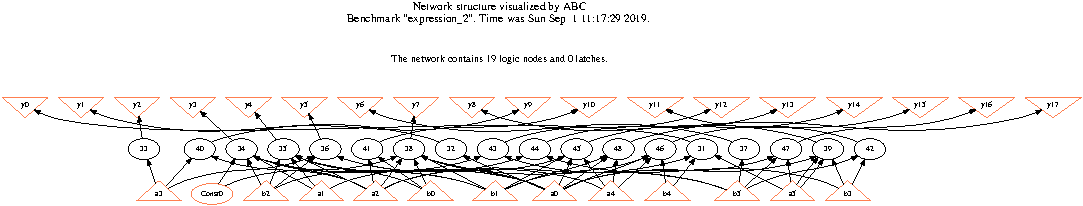
\includegraphics[scale=0.8]{MScThesisTemplate/Figs/expression_2.pdf}
    \caption{ \footnotesize General combinational circuit}
    \label{fig:expression}
\end{figure}
\subsection{Embedded circuit}
The synthesised netlist of ABC with \texttt{embedded.v} input shows in Fig.\ref{fig:embedded}. It can be observed that the sub-modules were separated into parts. Each sub-module has its only input/output logic. Based on circuit design block diagram \ref{fig:embedded}, all of the sub-modules are contained in a main-module. However, this hierarchy was automatically flatted by ABC and ABC will generate a warning that ''Can not detect external specification''. The size of an embedded circuit is around 1.9 kilobytes (82 line Verilog code).

This project only implemented one of the embedded hierarchy. The hierarchy can be complicated by increasing its level. For example, the sub-modules may locate at different levels. One sub-module has further contained its sub-sub-module. Besides, the output of a sub-module can be the input of another sub-module to complicate the generated circuit. The number of main-module could also be increased to extend the circuit complexity.

\begin{figure}[htb]
    \centering
    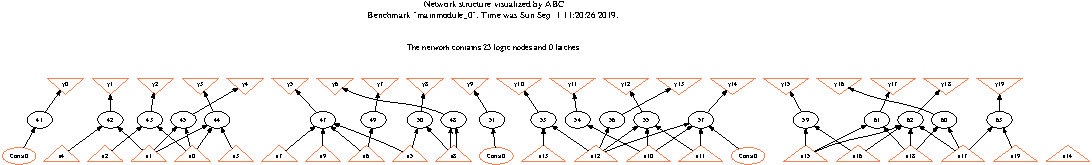
\includegraphics[width=14cm]{MScThesisTemplate/Figs/embedded_0.pdf}
    \caption{\footnotesize Embedded circuit}
    \label{fig:embedded}
\end{figure}

\subsection{Flip-flop}
The result of \texttt{flipflop.v} shows in Fig.\ref{fig:flipflop}. The size \texttt{flipflop.v} is the smallest, 32 bits (20 lines), among all kinds of circuits. Due to ABC's shortage in multi-bit processing, the structure of \texttt{flipflop.v} is comparative simple.  The rectangle represents the internal registers of the modules. The representation of input port and output port are the same with the combinational circuit.
\begin{figure}[htb]
    \centering
    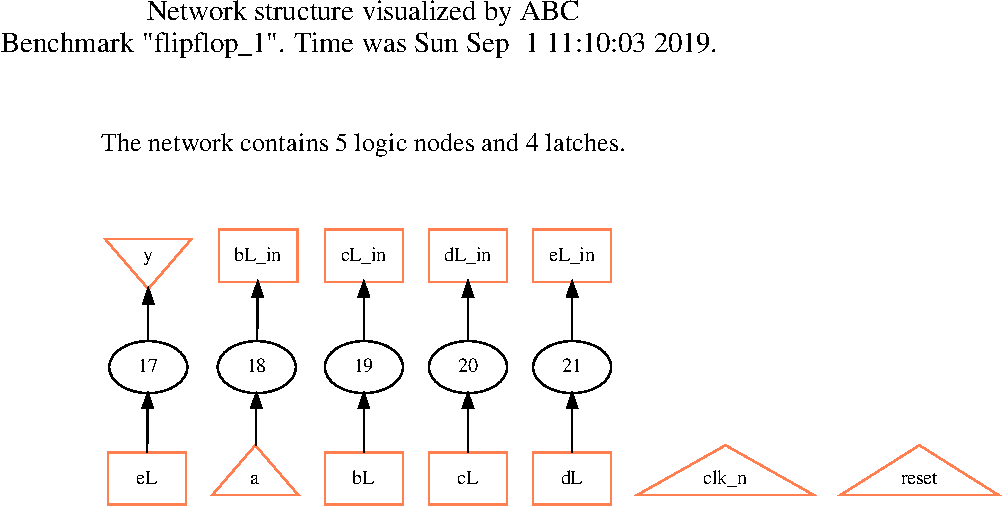
\includegraphics[width=14cm]{MScThesisTemplate/Figs/flipflop_1.pdf}
    \caption{ \footnotesize Sequential flip-flop circuit}
    \label{fig:flipflop}
\end{figure}

\subsection{Finite state machine}
Unfortunately, ABC can not synthesis the \texttt{FSM.v}. Because, states of an FSM need to be encoded in one-hot encoding method or binary encoding method \cite{golson1994state, harris2015digital}. These encoded states are stored in multi-bit registers. However, multi-bit is not supported by ABC. The size of this circuit is about 1 kilobyte (80 lines).

Although \texttt{FSM.v} can not be synthesised, the design of this kind of circuit provides a precursor in random sequential circuit generation. This circuit could be synthesised by other synthesis tools such as Icarus and VeriWell. It proves that the generated statements are valid and synthesisable.

\section{Algorithm analysis}
In order to analyse the time complexity of grey-box fuzzer, the runtime of generations was measured. The required number of generation was gradually increased from 10 files to 100,000 files. The scatter diagram of different kinds of circuits was plotted in Fig.\ref{Fig.sub.1}. The RHS figure is the space consumption diagram of the corresponding generation. It can be observed that \texttt{embedded.v} has the longest runtime and \texttt{FSM.v} consumes larget space under the same required number of file generation. The relative rate of growth in time and space are acceptable. It costs at most 8s to generate 100,000 random Verilog files.

\begin{figure}[htbp]
\centering
\label{Fig.sub.1}
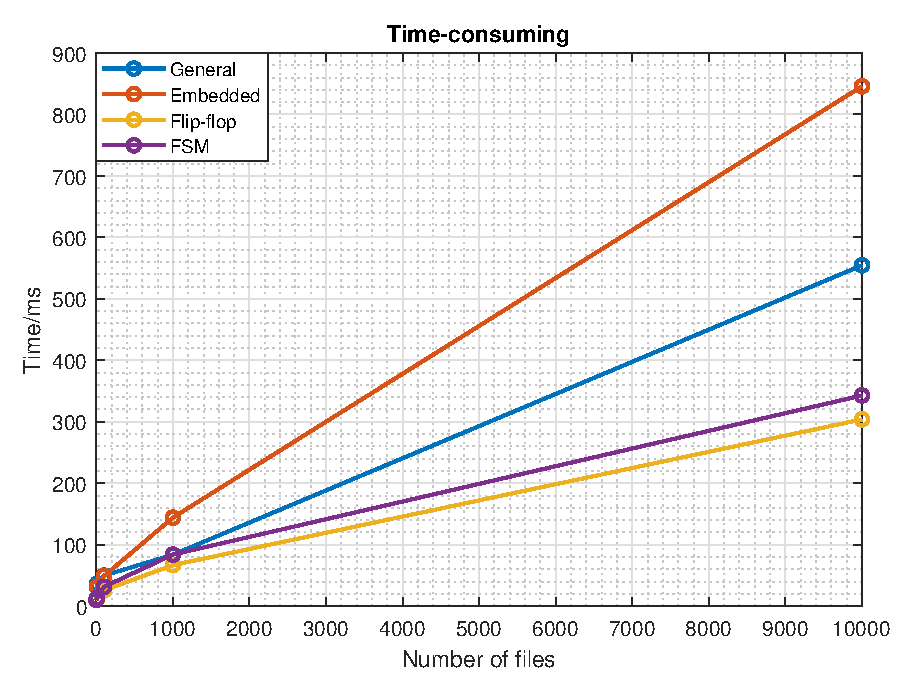
\includegraphics[width=10cm]{MScThesisTemplate/Figs/time.eps}
\end{figure}
Based on algorithm analysis \cite{allen2007data}, time complexity of an algorithm only calculate the upper bounded $O$ and discard lower order term and constant coefficient. As result, the algorithm analysis of this grey-box fuzzer focus on generation of \texttt{embedded.v} file. The time complexity analysis result of other generation is show in following table.
\begin{table}[htbp]
    \centering
    \begin{tabular}{c|c|c|c}
    \hline
         &  \texttt{general.v}&\texttt{flipflop.v}&\texttt{FSM.v}\\
    \hline
         Unbounded&$O(N^2)$&$O(N)$&$O(N^3)$\\
\hline
         Practical&$O(N)$&$O(N)$&$O(N)$\\
         \hline
    \end{tabular}
    \caption{Time complexity}
    \label{tab:tc}
\end{table}
The generation of grey-box fuzzer is full of uncertainty. As discussed in the evaluation strategy chapter \ref{prob}, the expected value is used in algorithm analysis. \texttt{Embedded.v} has two random variables, number of sub-modules and number of ports. It induces that the generation process has two degrees of freedom. An embedded ''for'' loop is required to conduct printing this circuit. If two random variables are unlimited ($\infty$), the upper bound of this algorithm is $O(N^{2})$. The recursive printing function of e\texttt{embedded.v} has $\frac{1}{5}$ to enter the recursion case (case ''? : '') and self-calling three times. The formed series is:
\begin{equation}
P_{1}=\frac{3}{5}, P_{2}=(\frac{3}{5})^2...P_{n}=(\frac{3}{5})^n
\end{equation}
\begin{equation}
\sum_{n=0}^{\infty}(\frac{3}{5})^{n} = \frac{1-(\frac{3}{5})^\infty}{1-\frac{3}{5}} = \frac{5}{2}
\end{equation}

It is convergent series and the final item $P_{n}$ converges to 0. With the help of dumping variable (/3 in each recursion), the rate of convergence becomes faster. It indicates that the complexity of recursion printing is $O(1)$. With the outer loop to perform file allocation, the total complexity of generating infinite files ($N \to\infty$) is $O(N_{3})$. In practice, two random variables are bounded within 10. Thus, the time complexity of \texttt{embedded.v} is $O(N)$. With the increasing of file number, time consumption is linearly increasing. The theoretical analysis result is consistent with the practical measurement on Fig.\ref{Fig.sub.1}. The reason of is not exactly a straight line is a random selection of Verilog statements and the random number of ports and sub-modules.

\begin{figure}[htbp]
\centering
\label{Fig.sub.2}
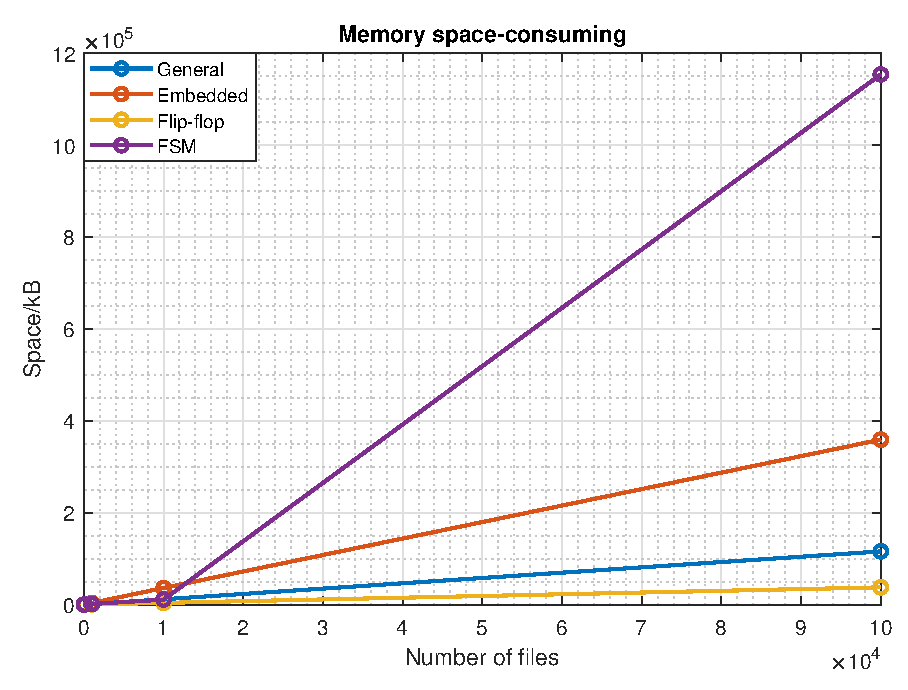
\includegraphics[width=10cm]{MScThesisTemplate/Figs/space.eps}
\caption{\footnotesize Algorithm analysis}
\end{figure}

Fig.\ref{Fig.port} and \ref{Fig.submodule} shows the runtime of the generation with changing of the number of ports and the number of sub-module. In order to avoid the random effect, the runtime is measured under 10,000 file generation. These two variables have a relation that total number ports equal ports of the number of sub-module times the number of ports on it.

\begin{equation}
    No.(ports) = No.(submodule) \times No.(port on it)
\end{equation}
When measuring the runtime of changing one variable, the other variable should remain as constant 1. The result shows that the time of adding sub-module generation (0.5) is longer than adding a port(0.025s). This result is reasonable because adding a sub-module requires more Verilog statements in the declaration. It is linear increasing, and the fluctuation is due to its randomness.

\begin{figure}[htbp]
\centering
\subfigure[port]{
\label{Fig.port}
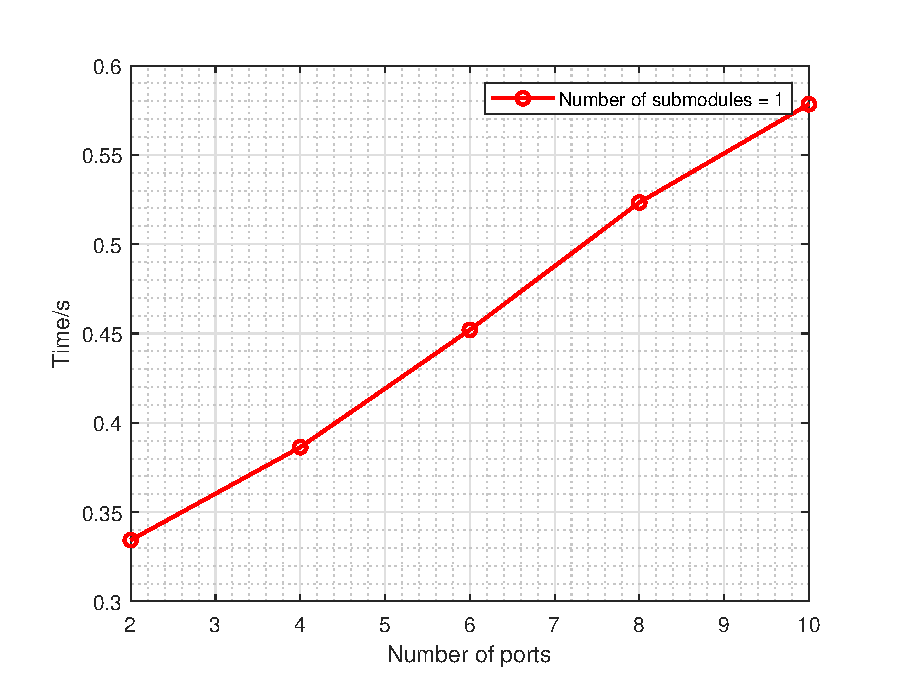
\includegraphics[width=0.5\textwidth]{MScThesisTemplate/Figs/port.eps}}
\subfigure[sub-module]{
\label{Fig.submodule}
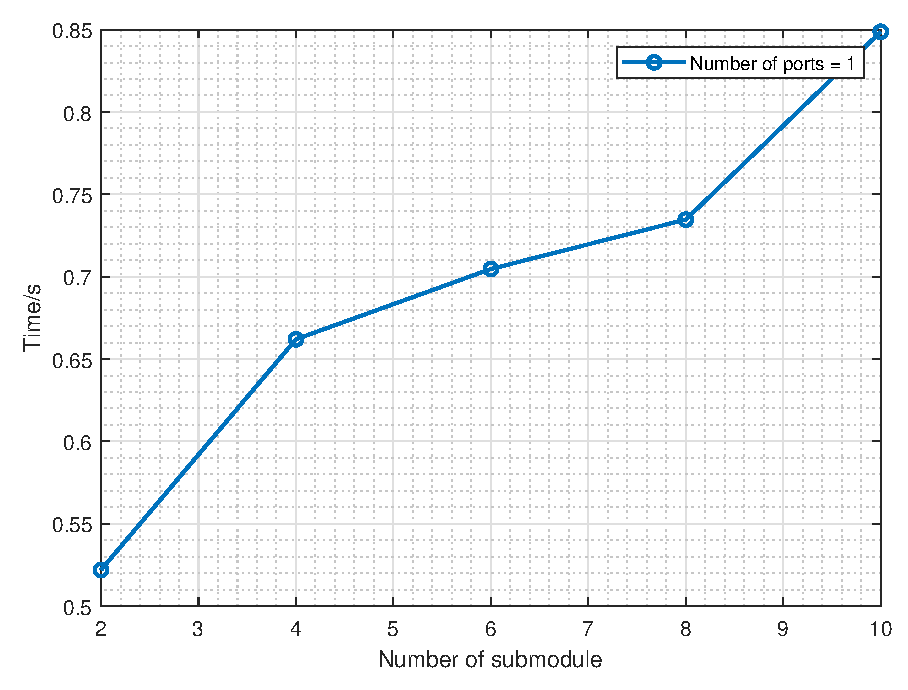
\includegraphics[width=0.45\textwidth]{MScThesisTemplate/Figs/submodule.eps}}
\caption{\footnotesize Algorithm analysis in change Number of port and Number of sub-module}
\end{figure}
For designed tool-flow script, the complexity is $O(N)$. Because it only contains one layer of ''for'' loop. The red line shows the runtime of ABC checking the script and the blue line shows the ABC and SIS checking script. However, SIS will be stuck when executing in batch mode. As a result, the blue line in the figure only contains runtime of adding a format converter. The result shows that the time consumption of ABC and SIS checking architecture is larger than ABC only checking architecture. If SIS can enter its batch mode, it will require even more time.  Time consumption of these two scripts under 10000 files execution is in a range of 4m57s to 6m4s. 
\begin{figure}[htbp]
    \centering
    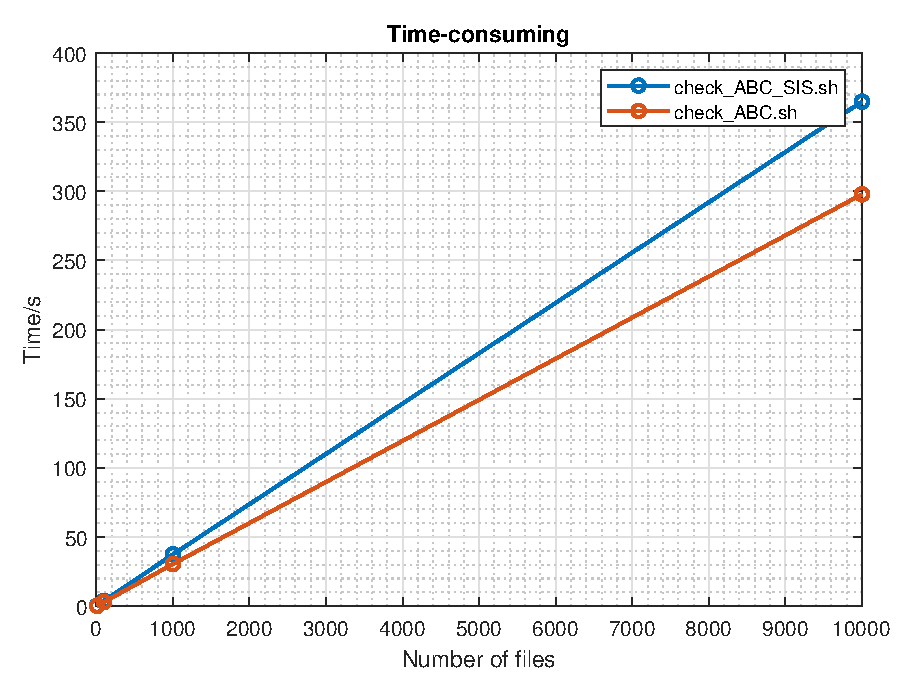
\includegraphics[width=10cm]{MScThesisTemplate/Figs/loop.eps}
    \caption{Tool-flow time consumption}
    \label{fig:loop}
\end{figure}


